\documentclass{../llncs}
%%%%%%%%%%%%%%%%%%%%%%%%%%%%%%%%%%%%%%%%%%%%%%%%%%%%%%%%%%%
%% package sillabazione italiana e uso lettere accentate
% \usepackage[latin1]{inputenc}
\usepackage[utf8]{inputenc}
\usepackage[english]{babel}
\usepackage[T1]{fontenc}
%%%%%%%%%%%%%%%%%%%%%%%%%%%%%%%%%%%%%%%%%%%%%%%%%%%%%%%%%%%%%

% per gli elenchi
\usepackage{enumitem}

% https://en.wikibooks.org/wiki/LaTeX/Source_Code_Listings
%%%%%%%%%%%%%%%%%%%%%%%%%%%%
\usepackage{listings}

\usepackage{xcolor}
\definecolor{darkgreen}{HTML}{007700}

\lstdefinestyle{style_qa}{
basicstyle=\small\ttfamily, columns=fullflexible,
keywordstyle=\color{violet}\bfseries, commentstyle=\color{darkgreen},
language=C++, breaklines=true,	 % sets automatic line breaking
captionpos=b,					 % sets the caption-position to bottom
morekeywords={Plan,System,Event,Dispatch,Context,ip,host,port,-httpserver,QActor,context,
normal,switchTo,transition,whenMsg,finally,repeatPlan,stopAfter,resumeLastPlan,
onMsg,addRule,replyToCaller,onEvent,removeRule,javaRun,whenTime,sendto,emit,else,not,
selfMsg,forward,delay,whenEvent,printCurrentEvent},
stringstyle=\color{blue},     	 % string literal style
caption={\lstname},
% title=\lstname,                  % show the filename of files included with \lstinputlisting; also try caption instead of title
numbers=left, numberstyle=\tiny,
stepnumber=1, numbersep=5pt, frame=shadowbox % , float=*
}

\lstdefinestyle{style_java}{
basicstyle=\small\ttfamily, columns=fullflexible,
keywordstyle=\color{violet}\bfseries, commentstyle=\color{darkgreen},
language=Java, breaklines=true,	 % sets automatic line breaking
captionpos=b,					 % sets the caption-position to bottom
stringstyle=\color{blue},     	 % string literal style
caption={\lstname},
% title=\lstname,                  % show the filename of files included with \lstinputlisting; also try caption instead of title
numbers=left, numberstyle=\tiny,
stepnumber=1, numbersep=5pt, frame=shadowbox % , float=*
}


\lstnewenvironment{codice_qa}[1][]
{\lstset{style=style_qa, #1}}{}

% \begin{lstlisting}
% ...
% \end{lstlisting}

% \begin{codice_qa}[caption={Programma Blink, "Hello World!"}]
% ...
% \end{codice_qa}

% \lstinputlisting[language=Python, firstline=37, lastline=45]{source_filename.py}
% \lstinputlisting[style=style_qa]{code/robotClient.qa}
%%%%%%%%%%%%%%%%%%%%%%%%%%%%

\usepackage{url}
\usepackage{xspace}
\usepackage{color}
\makeatletter
%%%%%%%%%%%%%%%%%%%%%%%%%%%%%% User specified LaTeX commands.
\usepackage{../manifest}

\makeatother

% https://en.wikibooks.org/wiki/LaTeX/Hyperlinks
% LaTeXimpaziente: "Il pacchetto hyperref, che di regola va caricato per ultimo, crea i collegamenti ipertestualivall’interno del documento, rendendo cliccabili i riferimenti incrociati"
\usepackage{hyperref}

%%%%%%%
 \newif\ifpdf
 \ifx\pdfoutput\undefined
 \pdffalse % we are not running PDFLaTeX
 \else
 \pdfoutput=1 % we are running PDFLaTeX
 \pdftrue
 \fi
%%%%%%%
 \ifpdf
 \usepackage[pdftex]{graphicx}
 \else
 \usepackage{graphicx}
 \fi
%%%%%%%%%%%%%%%
 \ifpdf
 \DeclareGraphicsExtensions{.pdf, .jpg, .tif}
 \else
 \DeclareGraphicsExtensions{.eps, .jpg}
 \fi
%%%%%%%%%%%%%%%

\newcommand{\java}{\textsf{Java}}
\newcommand{\android}{\texttt{Android}}
\newcommand{\dsl}{\texttt{DSL}}
\newcommand{\jazz}{\texttt{Jazz}}
\newcommand{\rtc}{\texttt{RTC}}
\newcommand{\ide}{\texttt{Contact-ide}}
\newcommand{\xtext}{\texttt{XText}}
\newcommand{\xpand}{\texttt{Xpand}}
\newcommand{\xtend}{\texttt{Xtend}}
\newcommand{\pojo}{\texttt{POJO}}
\newcommand{\junit}{\texttt{JUnit}}

\newcommand{\action}[1]{\texttt{#1}\xspace}
\newcommand{\codescript}[1]{{\scriptsize{\texttt{#1}}}\xspace}
\newcommand{\code}[1]{{\color{blue}\small{\texttt{#1}}}}
\newcommand{\fname}[1]{{\small{\color{magenta}\texttt{#1}}}}
\newcommand{\node}{\textsf{NodeJs}}
\newcommand{\qa}{\textsf{\textit{QActor}}}

% Cross-referencing
\newcommand{\labelsec}[1]{\label{sec:#1}}
\newcommand{\xs}[1]{\sectionname~\ref{sec:#1}}
\newcommand{\xsp}[1]{\sectionname~\ref{sec:#1} \onpagename~\pageref{sec:#1}}
\newcommand{\labelssec}[1]{\label{ssec:#1}}
\newcommand{\xss}[1]{\subsectionname~\ref{ssec:#1}}
\newcommand{\xssp}[1]{\subsectionname~\ref{ssec:#1} \onpagename~\pageref{ssec:#1}}
\newcommand{\labelsssec}[1]{\label{sssec:#1}}
\newcommand{\xsss}[1]{\subsectionname~\ref{sssec:#1}}
\newcommand{\xsssp}[1]{\subsectionname~\ref{sssec:#1} \onpagename~\pageref{sssec:#1}}
\newcommand{\labelfig}[1]{\label{fig:#1}}
\newcommand{\xf}[1]{\figurename~\ref{fig:#1}}
\newcommand{\xfp}[1]{\figurename~\ref{fig:#1} \onpagename~\pageref{fig:#1}}
\newcommand{\labeltab}[1]{\label{tab:#1}}
\newcommand{\xt}[1]{\tablename~\ref{tab:#1}}
\newcommand{\xtp}[1]{\tablename~\ref{tab:#1} \onpagename~\pageref{tab:#1}}
% Category Names
\newcommand{\sectionname}{Section}
\newcommand{\subsectionname}{Subsection}
\newcommand{\sectionsname}{Sections}
\newcommand{\subsectionsname}{Subsections}
\newcommand{\secname}{\sectionname}
\newcommand{\ssecname}{\subsectionname}
\newcommand{\secsname}{\sectionsname}
\newcommand{\ssecsname}{\subsectionsname}
\newcommand{\onpagename}{on page}

\newcommand{\xauthA}{Filippo Frabetti}
\newcommand{\xauthB}{Nicola Semprini}
\newcommand{\xauthC}{Paolo Magnani}
\newcommand{\xfaculty}{II Faculty of Engineering}
\newcommand{\xunibo}{Alma Mater Studiorum -- University of Bologna}
\newcommand{\xaddrBO}{viale Risorgimento 2}
\newcommand{\xaddrCE}{via Venezia 52}
\newcommand{\xcityBO}{40136 Bologna, Italy}
\newcommand{\xcityCE}{47023 Cesena, Italy}

%
% Comments
%
% What’s wrong with \bf, \it, etc.? --> https://texfaq.org/FAQ-2letterfontcmd
% \newcommand{\todo}[1]{\bf{TODO:}\emph{#1}}
\newcommand{\todo}[1]{\textbf{TODO:} \emph{#1}}

\begin{document}

\title{Software Systems Engineering: Final task 2018}

\author{\xauthA, \xauthB, \xauthC}

\institute{%
  \xunibo\\\xaddrBO, \xcityBO\\
  \email{filippo.frabetti@studio.unibo.it}\\
  \email{nicola.semprini4@studio.unibo.it}\\
  \email{paolo.magnani5@studio.unibo.it}
}

\maketitle

% %%%%%%%%%%%%%%%%%%%%%%%% ABSTRACT + KEYWORDS - TODO... %%%%%%%%%%%%%%%%%%%%%%%%
\begin{abstract}
\footnotesize

This document is the explicit representation of the production process adopted.\\

\todo{abstract and keywords}

% (This part is optional)
%%This a Latex template to be used for the explicit representation of the production process adopted in the Software Systems Engineering course. 
% THIS DOCUMENT MUST FILL AT MOST TWO PAGES AND MUST BE PRINTED ON A SINGLE PAPER SHEET.

% The document can be compiled by using the \fname{kitISLatex.zip} given in \code{iss2018/it.unibo.issMaterial/issdocs/Lab}
  
\keywords{
% (This part is optional)
Software engineering, software development process, process representation, ...
}
\end{abstract}

\sloppy

%===========================================================================
\section{Introduction}
\labelsec{intro}
%===========================================================================

%===========================================================================
\section{Vision}
\labelsec{vision}

Scegliamo di procedere top-down, con zooming progressivo verso i dettagli.
%=========================================================================== 

%===========================================================================
\section{Requirements}
\labelsec{Requirements}

%With reference to a \texttt{mbot} physical robot working in a virtual environment, build an application that sends the data sensed by the virtual and the real sonars to the radar. More specifically:
%\begin{itemize}
%\item[-]the data of the \emph{virtual sonar} \texttt{sonar1} must be displayed on the direction of angle=\fname{30};
%\item[-]the data of the \emph{virtual sonar} \texttt{sonar2} must be displayed on the direction of angle=\fname{120};
%\item[-]the data of the \emph{virtual sonar} on the virtual robot must be displayed on the direction of angle=\fname{90} at the fixed distance of \fname{40};
%\item[-]the data of the \emph{real sonar} on the physical robot must be displayed on the direction of angle=\fname{0};
%\end{itemize}

% 13 - A new problem
%\begin{enumerate}
%\item The physical robot must expose in a visible way a \code{Led} and:
%\begin{itemize}
%\item[-] the Led must be \code{on} when the robot is engaged by an user (human or machine);
%\item[-] the Led must be \code{off} when the robot is available for booking.
%\end{itemize}
%\item the robot system does not expose any public available usage interface;
%\item in order to use the robot, an user must first of all send 'to the system' a \code{booking request}. The system
%must return an answer including an \code{access token} if the robot is available. If the answer is negative, (robot
%already engaged) and the request includes a '\texttt{notify-me flag}', the system must notify the user when to robot
%becomes again available;
%\item the user that receives the \code{access token} must send within a given \code{acquisition-deadline} (e.g. \code{30 sec}) the request for a \emph{robot-driving command interface}, by appending to the request the \code{access token}. If the
%\emph{acquisition-deadline} expires, the robot returns in its 'available state';
%\item the user can use the \emph{robot-driving command interface} at most for a prefixed \code{usage-duration} time;
%\item the user can explicitly release the robot resource by sending a \code{booking release} message;
%\item if many users attempt to book the robot resource 'at the same time', the system could operate in two different
%ways:
%\begin{itemize}
%\item[(a)] by selecting the first \emph{emitted} request;
%\item[(b)] by selecting the first \emph{received} request
%\end{itemize}
%\end{enumerate}

% FINAL TASK 2018
In a home of a given city (e.g. Bologna), a \texttt{ddr} robot is used to clean the floor of a room (\code{R-FloorClean}).

The floor in the room is a flat floor of solid material and is equipped with two \emph{sonars}, named \code{sonar1} and \code{sonar2} as shown in the picture (\code{sonar1} is that at the top). The initial position (\code{start-point}) of the robot is detected by \code{sonar1}, while the final position (\code{end-point}) is detected by \code{sonar2}.\\

The robot works under the following conditions:
\begin{enumerate}
\item \code{R-Start}: an \code{authorized user} has sent a \texttt{START} command by using a human \texttt{GUI} interface (\code{console}) running
on a conventional PC or on a smart device (\texttt{Android}).
\item \code{R-TempOk}: the value temperature of the city is not higher than a prefixed value (e.g. \texttt{25} degrees Celsius).
\item \code{R-TimeOk}: the current clock time is within a given interval (e.g. between \texttt{7} a.m and \texttt{10} a.m )
\end{enumerate}

While the robot is working:
\begin{itemize}[label={--}]
\item it must blink a \texttt{Led} put on it, if the robot is a \fname{real} robot (\code{R-BlinkLed}).
\item it must blink a \texttt{Led Hue Lamp} available in the house, if the robot is a \fname{virtual} robot (\code{R-BlinkHue}).
\item it must avoid fixed obstacles (e.g. furniture) present in the room (\code{R-AvoidFix}) and/or mobile obstacles like
balls, cats, etc. (\code{R-AvoidMobile}).
\end{itemize}

Moreover, the robot must stop its activity when one of the following conditions apply:
\begin{enumerate}
\item \code{R-Stop}: an \code{authorized user} has sent a \texttt{STOP} command by using the \code{console}.
\item \code{R-TempKo}: the value temperature of the city becomes higher than the prefixed value.
\item \code{R-TimeKo}: the current clock time is beyond the given interval.
\item \code{R-Obstacle}: the robot has found an obstacle that it is unable to avoid.
\item \code{R-End}: the robot has finished its work.
\end{enumerate}

%During its work, the robot can optionally:
%\begin{itemize}[label={--}]
%\item \code{R-Map}: build a map of the room floor with the position of the fixed obstacles. Once built, this map can be
%used to define a plan for an (optimal) path form the \code{start-point} to the \code{end-point}.
%\end{itemize}
%
%Other requirements:
%\begin{enumerate}
%\item The work can be done by a team composed of \code{NT} people, with \code{1<=NT<=4}.
%\item If \code{NT>1}, the team must explicitly indicate the work done by each component.
%\item If \code{NT==4}, the requirement \code{R-Map} is mandatory.
%\end{enumerate}
%===========================================================================

%===========================================================================
\section{Requirement analysis}
\labelsec{ReqAnalysis}

Dai requisiti si delineano 6 entità:
\begin{enumerate}
\item il robot, che può essere sia fisico sia virtuale (\texttt{RealDDR} e \texttt{VirtualDDR})
\item l'ambiente in cui si muove (fisico/virtuale) %, a sua volta costituito da:
%	\begin{itemize}
%	\item 2 sensori (\code{sonar1} e \code{sonar2})
%	\item ostacoli fissi (pareti) e mobili
%	\end{itemize}
\item gli attuatori: il \texttt{Led} per il robot reale e l'\texttt{Hue Lamp} per quello virtuale
\item i sensori remoti: un indicatore di temperatura (\texttt{TemperatureSensor}) e un orologio (\texttt{Clock})
\item un utilizzatore umano (\texttt{HumanOperator})
\item più un componente che andrà ad incapsulare l'\texttt{Application logic}
\end{enumerate}

L'ambiente è inoltre costituito a sua volta da:
\begin{itemize}[label={--}]
\item 2 sensori \code{sonar1} e \code{sonar2} (ambiente virtuale)
\item ostacoli fissi (pareti) e mobili
\end{itemize}

L'architettura del sistema può essere descritta in maniera informale dalla \xf{informalRA}.
\begin{figure}[!htb]
\centering
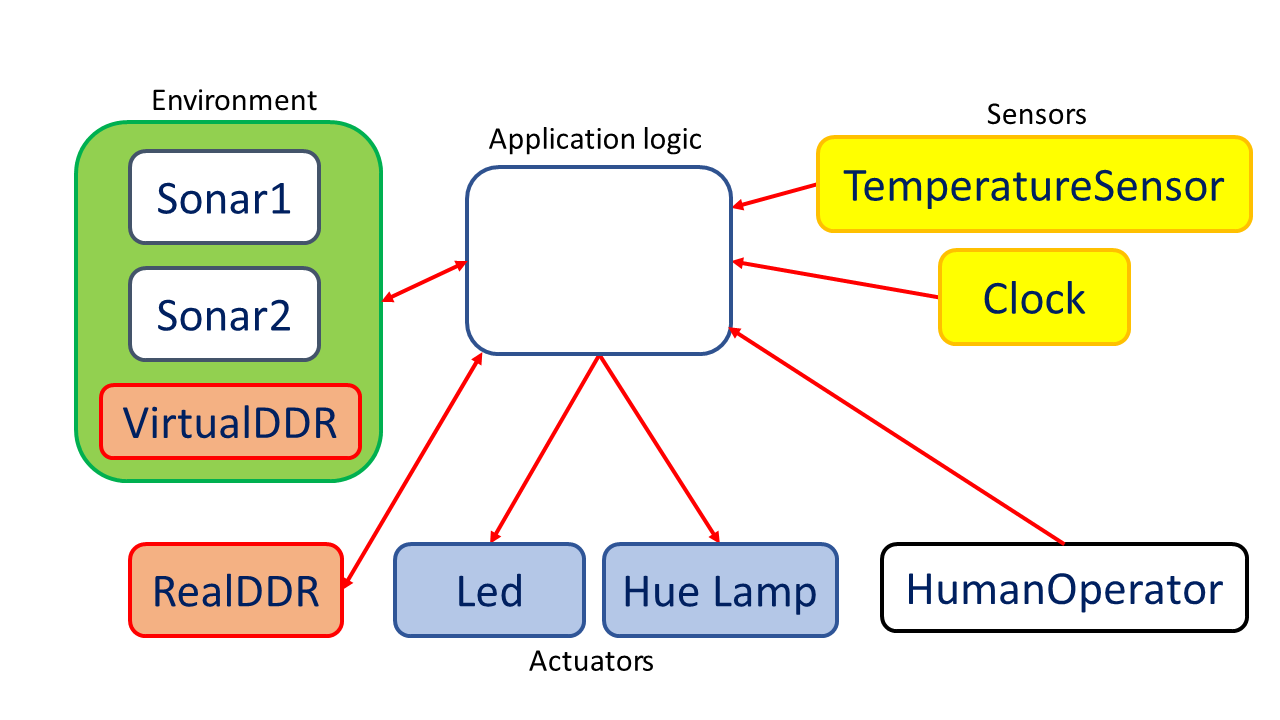
\includegraphics[scale=0.4]{img/informalReqAnalysis.png}
\caption{Architettura informale ottenuta dall'analisi dei requisiti}\labelfig{informalRA}
\end{figure}

\subsection{Actuators}
Il \texttt{Led}, essendo un'entità passiva senza un proprio flusso di controllo, è possibile modellarlo come un oggetto Java che implementi la seguente interfaccia:\\

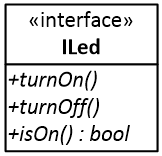
\includegraphics[scale=0.4]{img/iled.png}

L'\texttt{Hue Lamp} è invece un'entità attiva che ci viene fornita dal committente insieme ad un componente software per poter interagire con essa attraverso un'interfaccia \textit{RESTful}
\footnote{link doc page}.

Possiamo quindi definire il modello di un attore in grado di interagire con l'\texttt{Hue Lamp}. Per farlo usiamo il linguaggio custom della nostra Software House \qa, poiché ci permette di modellare sistemi distribuiti eterogenei.\\

\lstinputlisting[style=style_qa]{../it.unibo.finalTask2018/src/hueLampAgent.qa}

Si noti come la scelta di utilizzare l'evento \codescript{blinkCmd} consente di far \textit{lampeggiare} più dispositivi senza che questi siano noti a priori dalla sorgente che emette tali eventi in base alla logica applicativa.

\subsection{Sensors}
Poiché abbiamo a che fare con sensori remoti, ci viene naturale modellarli come attori che rendono disponibili delle informazioni espresse in un certo formato.

Nello specifico, sono possibili due approcci:
\begin{itemize}
\item a polling, ovvero è chi necessita dell'informazione a farsi carico di fare richiesta periodicamente al sensore
\item oppure può essere il sensore stesso a pubblicare all'esterno le informazioni quando queste sono disponibili 
\end{itemize}
Scegliamo di adottare questa seconda strategia, poiché meno costosa in termini di dati scambiati e poiché garantisce un minor accoppiamento tra le entità coinvolte.

Anche in questo caso il sensore, non conoscendo i componenti interessati, emette un evento che può essere percepito da chiunque sia in ascolto.\\

\lstinputlisting[style=style_qa]{../it.unibo.finalTask2018/src/temperatureAgent.qa}

Si riportano solo le variazioni essenziali per il \texttt{Clock}:

\lstinputlisting[style=style_qa, firstline=13, lastline=20, firstnumber=13]{../it.unibo.finalTask2018/src/clockAgent.qa}

\subsection{DDR}
Ci viene fornito un modello del robot virtuale espresso nel linguaggio \qa
\footnote{percorso file}
: questi è in grado di ricevere messaggi \codescript{moveRobot : moveRobot( CMD )} e di interpretarli come comandi di movimento (stop, forward, left, right, backward).

Il robot è quindi un'entità attiva il cui scopo è interpretare i messaggi ricevuti in un certo formato. L'implementazione delle varie mosse è delegata ad un'opportuna classe Java che può essere modificata senza alterare il modello del robot.\\

\lstinputlisting[style=style_qa]{../it.unibo.finalTask2018/src/robotDDR.qa}

\subsection{HumanOperator}
Lo \texttt{HumanOperator} può essere modellato come un emettitore di comandi per il robot. In realtà, per disaccoppiare le comunicazioni tra sorgente e destinatario dei comandi, l'operator si rivolge ad una terza entità, che rappresenta la logica applicativa, così che non sia vincolato a conoscere l'identità di ogni possibile robot pilotabile.\\

\lstinputlisting[style=style_qa]{../it.unibo.finalTask2018/src/humanOperator.qa}

Per un primo testing, l'intermediario dei messaggi è un attore \codescript{testapplqa} che si trova nello stesso contesto dell'operator. In futuro, quest'ultimo dovrà conoscere il contesto dell'entità che rappresenta la logica applicativa, così da poterle inviare messaggi (vedi riga 6).

\subsection{Environment}
Nell'ambiente virtuale sono presenti i due sonar in grado di rilevare la presenza di un robot che passi in corrispondenza di uno dei due. Per questo motivo, l'ambiente stesso può essere visto alla stregua di un ulteriore sensore che emette eventi \codescript{sonarSensor}.\\

\lstinputlisting[style=style_qa]{../it.unibo.finalTask2018/src/virtualEnvironment.qa}

Da notare come l'emissione di tali eventi dipenda dalla specifica implementazione del \textit{virtual environment}:

\lstinputlisting[style=style_java, firstline=7, lastline=17, firstnumber=7]{../it.unibo.finalTask2018/src/it/unibo/finalTask2018/adapter/envAdapter.java}

\subsection{Application logic}
La nostra applicazione, oltre ad incapsulare le politiche della logica applicativa, deve innanzitutto agire come \textit{"system integrator"}, mettendo in collegamento i vari componenti così che questi possano interagire.
Si noti infatti come ogni componente è stato fino ad ora modellato come un micro-servizio indipendente.\\

L'immagine della \xf{informalRA} può essere quindi formalmente definita dal seguente sistema {\qa}:\\

\lstinputlisting[style=style_qa]{../it.unibo.finalTask2018/src/reqAnalysisModel.qa}

In questo caso sensori, attuatori, operatori, ambiente e robot sono stati tutti inseriti all'interno di un unico contesto per motivi di rapidità di modellazione e di \textit{integration testing}.

Poiché abbiamo utilizzato un modello eseguibile, questo ci fornisce anche un primo prototipo funzionante della nostra applicazione.
%===========================================================================


%===========================================================================
\section{Problem analysis}
\labelsec{ProblemAnalysis}
%===========================================================================

%===========================================================================
\section{Project}
\labelsec{Project}
%===========================================================================

%===========================================================================
\section{Implementation}
\labelsec{Implementation}
%===========================================================================

%===========================================================================
\section{Testing}
\labelsec{Testing}
%===========================================================================

%===========================================================================
\section{Maintenance}
\labelsec{Maintenance}
%===========================================================================

%===========================================================================
\section{Deployment}
\labelsec{Deployment}
%===========================================================================
 
%===========================================================================
\section{Author}
\labelsec{Author}
%===========================================================================

\vskip.5cm
%%% \begin{figure}
\begin{tabular}{ | c |  }
\hline
  % after \\: \hline or \cline{col1-col2} \cline{col3-col4} ...
  Photo of the author 
  \\
\hline
   %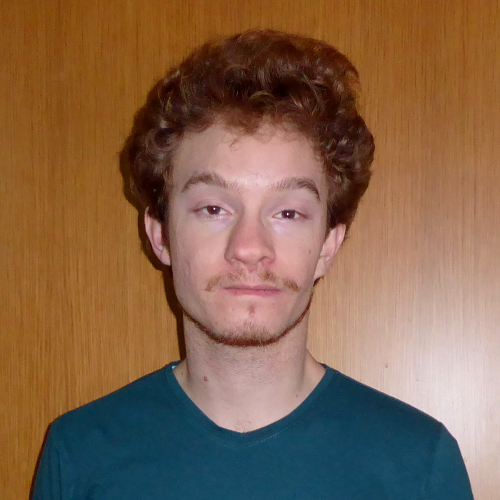
\includegraphics[scale = 0.7]{img/foto_autore.jpg}
   %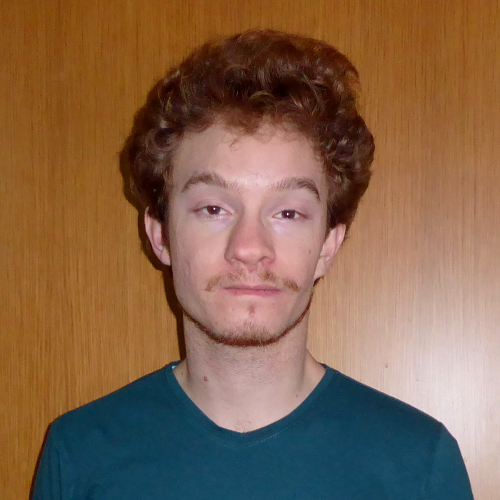
\includegraphics{img/foto_autore.jpg}
  \\
\hline
\end{tabular}
 
\end{document}
